\documentclass[a4paper, 12pt]{article}
% page
% \usepackage[top=2.54cm,bottom=2.54cm,left=3.18cm,right=3.18cm]{geometry}  % default
\usepackage{graphicx}
\usepackage[top=2.27cm,bottom=1.27cm,left=1.27cm,right=1.27cm]{geometry}
\usepackage[none]{hyphenat} % remove hyphen

% header and footer
\usepackage{fancyhdr}
\fancypagestyle{plain}{
    \fancyhead[L]{}
    \fancyhead[C]{Computer Vision HW1 Report}
    \fancyhead[R]{Student ID: R11625015\\ Name: 廖致豪}
    % \fancyfoot[L]{}
    % \fancyfoot[C]{}
    % \fancyfoot[R]{}
    \renewcommand{\headrulewidth}{0.5pt}
    \renewcommand{\footrulewidth}{0pt}
    \setlength{\headheight}{27.58636pt}
    \addtolength{\topmargin}{-0.28833pt}
}
\pagestyle{plain}

% font setting
\usepackage{fontspec}
\usepackage{xeCJK}
    \setCJKmainfont{標楷體}
    % \setCJKmainfont{微軟正黑體}
    \XeTeXlinebreaklocale "zh"
    \XeTeXlinebreakskip = 0pt plus 1pt
    \defaultCJKfontfeatures{AutoFakeBold=true,AutoFakeSlant=true}
    % \newCJKfontfamily\Kai{標楷體}
    \newCJKfontfamily\Hei{微軟正黑體}
    \newCJKfontfamily\NewMing{新細明體}
    \setmainfont{Arial}   % Set English to Arial

% codestyle
\usepackage{listings}
\usepackage{xcolor}
\definecolor{codegreen}{rgb}{0,0.6,0}
\definecolor{codegray}{rgb}{0.5,0.5,0.5}
\definecolor{codepurple}{rgb}{0.58,0,0.82}
\definecolor{backcolour}{rgb}{0.95,0.95,0.92}

\lstdefinestyle{mystyle}{
    backgroundcolor=\color{backcolour},   
    commentstyle=\color{codegreen},
    keywordstyle=\color{magenta},
    numberstyle=\tiny\color{codegray},
    stringstyle=\color{codepurple},
    basicstyle=\ttfamily\footnotesize,
    breakatwhitespace=false,         
    breaklines=true,                 
    captionpos=b,                    
    keepspaces=true,                 
    numbers=left,                    
    numbersep=5pt,                  
    showspaces=false,                
    showstringspaces=false,
    showtabs=false,                  
    tabsize=2
}

\lstset{style=mystyle}

% packages
\usepackage{tabularx, array, slashbox}
\usepackage{makecell}
\usepackage{multirow}
\usepackage{amsmath}
\usepackage{url}

% main page
\begin{document}
\section{Part 1}
\subsection{Visualize the DoG images of 1.png}
\begin{table}[!htb]
    \centering
    \caption{Visualizing DoG Images for 1.png and 2.png}
    \begin{tabular}{|c|c|c|c|}
        \hline
                   & DoG Image (threshold = 3)                           &            & DoG Image (threshold = 3)                             \\
        \hline
        DoG1-1.png & 
\includegraphics[scale=1]{part1/result/DoG_1_1.png} & DoG2-1.png & 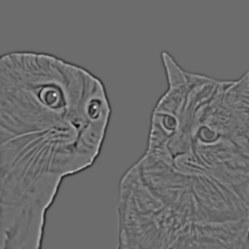
\includegraphics[scale=0.6]{part1/result/DoG_2_1.png} \\
        \hline
        DoG1-2.png & 
\includegraphics[scale=1]{part1/result/DoG_1_2.png} & DoG2-2.png & 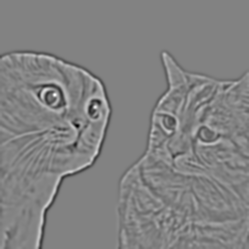
\includegraphics[scale=0.6]{part1/result/DoG_2_2.png} \\
        \hline
        DoG1-3.png & 
\includegraphics[scale=1]{part1/result/DoG_1_3.png} & DoG2-3.png & 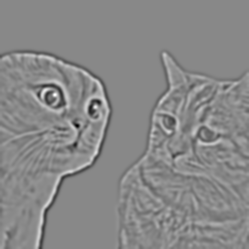
\includegraphics[scale=0.6]{part1/result/DoG_2_3.png} \\
        \hline
        DoG1-4.png & 
\includegraphics[scale=1]{part1/result/DoG_1_4.png} & DoG2-4.png & 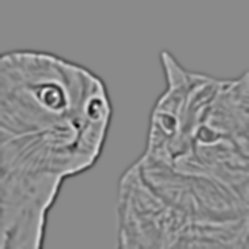
\includegraphics[scale=0.6]{part1/result/DoG_2_4.png} \\
        \hline
    \end{tabular}
\end{table}

\subsection{Use three thresholds (1,2,3) on 2.png and describe the difference}
\begin{table}[!htb]
    \centering
    \caption{Keypoints detected on 2.png with three thresholds}
    \begin{tabular}{|c|c|}
        \hline
        Threshold & Image with detected keypoints on 2.png                         \\
        \hline
        1         & 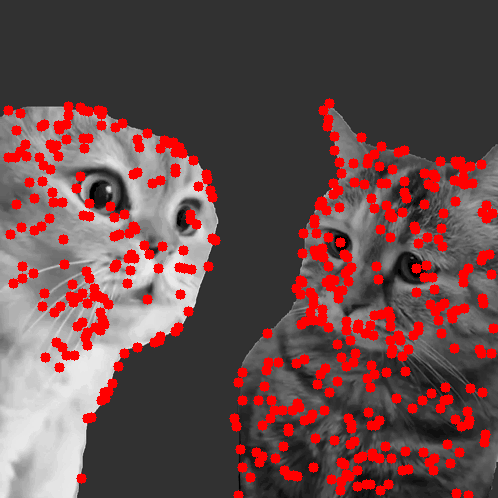
\includegraphics[scale=0.4]{part1/result/DoG_2_1.0_result.png} \\
        \hline
        2         & 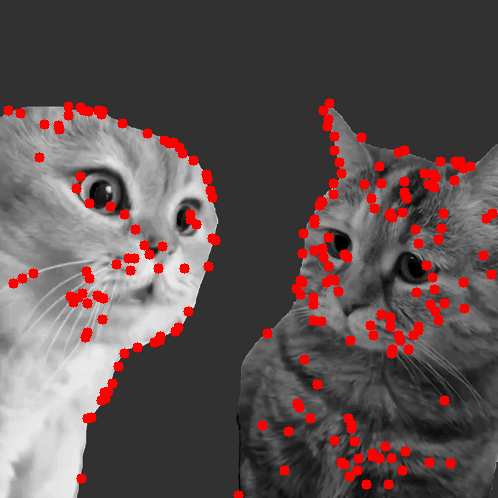
\includegraphics[scale=0.4]{part1/result/DoG_2_2.0_result.png} \\
        \hline
        3         & 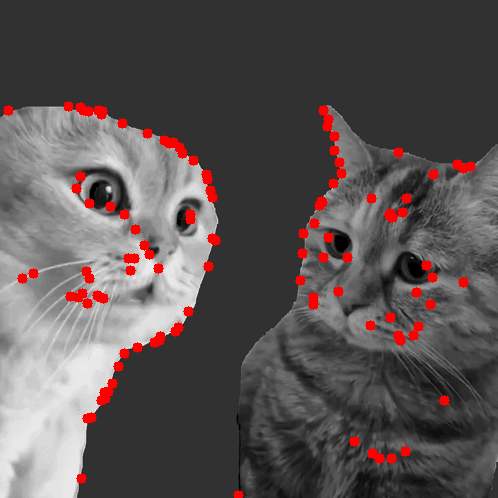
\includegraphics[scale=0.4]{part1/result/DoG_2_3.0_result.png} \\
        \hline
    \end{tabular}
\end{table}

\clearpage

\begin{center}
    \textbf{(describe the difference)}
\end{center}

By plotting the Difference of Gaussians (GoG) features on 2.png using three distinct threshold values (1, 2, 3), it becomes apparent that lower thresholds yield a great number of key points, whereas higher thresholds lead to a reduction in the number of detected key points. The keypoints are predominantly concentrated in the foreground rather than the background regions of the image because the colors in cat's body exhibit richer variation comared to the background color. Additionally, keypoints with higher levels of contrast receive more weighting, while keypoints with lower contrast may prone to being assotiated with noise points. Consequently, in instances where higher thresholds are applied, some keypoints on the cat's bodies may be omitted and filtered out, leaving predominately those points far from the background with more pronounced gradients, and noise points will be remoed from the keypoints list.

\section{Part 2}
\subsection{Report the cost for each filtered image}
\begin{table}[!htb]
    % \caption{Global caption}
    \centering
    \begin{minipage}{.5\linewidth}
        \caption{Cost evaluation for 1.png}
        \centering
        \begin{tabular}{|c|c|}
            \hline
            Gray Scale Setting  & Cost (1.png) \\
            \hline
            cv.2COLOR\_BGR2GRAY & 1207799      \\
            \hline
            R*0.0+G*0.0+B*1.0   & 1439568      \\
            \hline
            R*0.0+G*1.0+B*0.0   & 1305961      \\
            \hline
            R*0.1+G*0.0+B*0.9   & 1393620      \\
            \hline
            R*0.1+G*0.4+B*0.5   & 1279697      \\
            \hline
            R*0.8+G*0.2+B*0.0   & 1127913      \\
            \hline
        \end{tabular}
    \end{minipage}%
    \begin{minipage}{.5\linewidth}
        \centering
        \caption{Cost evaluation for 2.png}
        \begin{tabular}{|c|c|}
            \hline
            Gray Scale Setting  & Cost (2.png) \\
            \hline
            cv2.COLOR\_BGR2GRAY & 183850       \\
            \hline
            R*0.1+G*0.0+B*0.9   & 77882        \\
            \hline
            R*0.2+G*0.0+B*0.8   & 86023        \\
            \hline
            R*0.2+G*0.8+B*0.0   & 188019       \\
            \hline
            R*0.4+G*0.0+B*0.6   & 128341       \\
            \hline
            R*1.0+G*0.0+B*0.0   & 110862       \\
            \hline
        \end{tabular}
    \end{minipage}
\end{table}

\subsection{Show original RGB image / two filtered RGB images and two grayscale images with highest and lowest cost.}
\begin{table}[!htb]
    \centering
    \caption{Comparing origin and filtered images with different costs on 1.png}
    \begin{tabular}{|c|p{0.3\linewidth}|p{0.3\linewidth}|}
        \hline
        Original RGB image (1.png)                        & Filtered RGB image and Grayscale image of Highest cost               & Filtered RGB image and Grayscale image of Lowest cost                \\
        \hline
        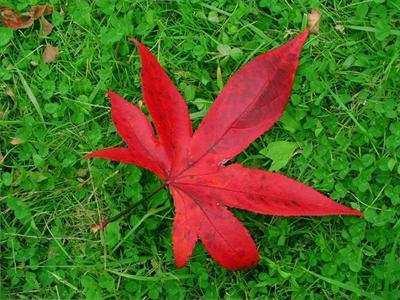
\includegraphics[scale=0.4]{part2/testdata/1.png} & 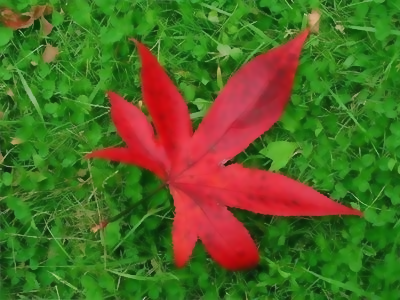
\includegraphics[scale=0.4]{part2/result/1_RGB_0.0_0.0_1.0_JBF.png}  & 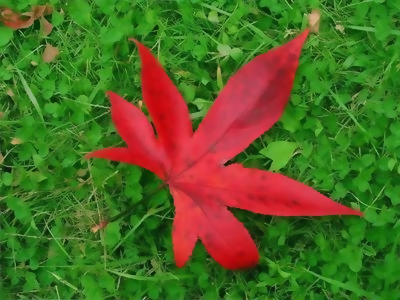
\includegraphics[scale=0.4]{part2/result/1_RGB_0.8_0.2_0.0_JBF.png}  \\
        \hline
        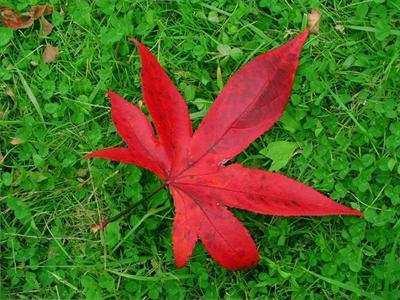
\includegraphics[scale=0.4]{part2/testdata/1.png} & 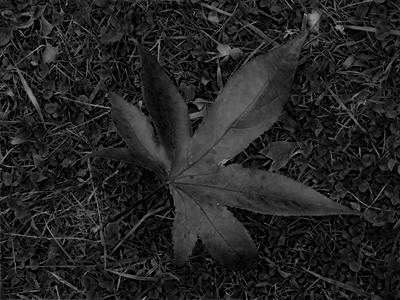
\includegraphics[scale=0.4]{part2/result/1_RGB_0.0_0.0_1.0_gray.png} & 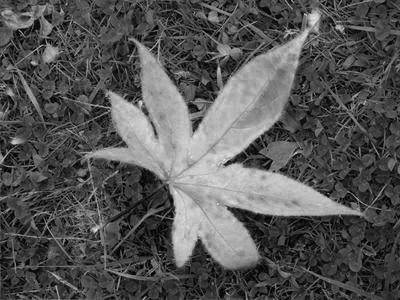
\includegraphics[scale=0.4]{part2/result/1_RGB_0.8_0.2_0.0_gray.png} \\
        \hline
    \end{tabular}
\end{table}

\begin{center}
    \textbf{(Describe the difference between those two grayscale images)}
\end{center}

Upon examining Table 3, it becomes apparent that the combination yielding a higher cost is $R*0.0+G*0.0+B*1.0 (1439568)$, while the one with a lower cost is $R*0.8+G*0.2+B*0.0(1127913)$. Since the predominant presence of red and green hues in the image, if the combination heavily favors blue or colors outside the color gamut during the RGB to YUV color space conversion, it may incur higher costs, and the brightness of the grayscale images will be diminished, leading to a suboptimal transformation in the final images. Although noise reduction is achieved, the image quality appears somewhat blurred. Conversely, the lower-cost combination utilizes weights from red and green, which are more prevalent in the image, resulting in a smaller mean shift and brighter overall brightness. This combination demonstrates better performance in the outcome image, ultimately delivering noise-free details on the original image.

\begin{table}[!htb]
    \centering
    \caption{Comparing origin and filtered images with different costs on 2.png}
    \begin{tabular}{|c|p{0.3\linewidth}|p{0.3\linewidth}|}
        \hline
        Original RGB image (2.png)                        & Filtered RGB image and Grayscale image of Highest cost               & Filtered RGB image and Grayscale image of Lowest cost                \\
        \hline
        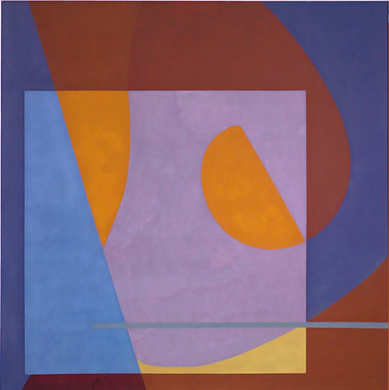
\includegraphics[scale=0.5]{part2/testdata/2.png} & 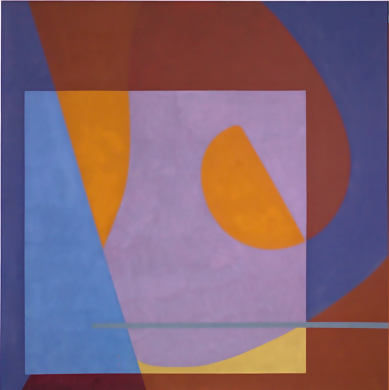
\includegraphics[scale=0.4]{part2/result/2_RGB_0.2_0.8_0.0_JBF.png}  & 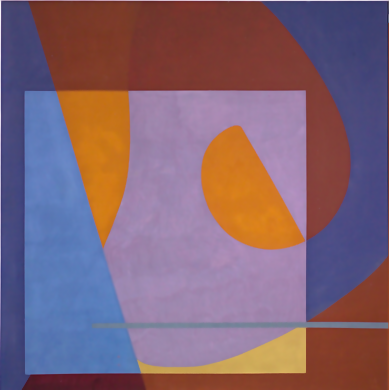
\includegraphics[scale=0.4]{part2/result/2_RGB_0.1_0.0_0.9_JBF.png}  \\
        \hline
        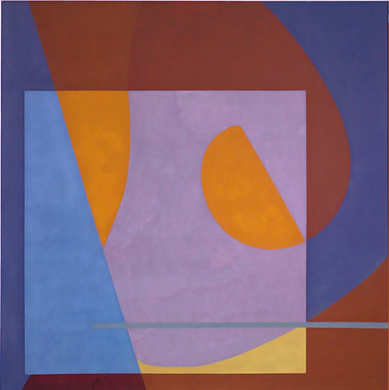
\includegraphics[scale=0.5]{part2/testdata/2.png} & 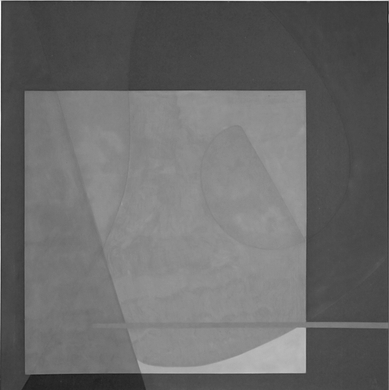
\includegraphics[scale=0.4]{part2/result/2_RGB_0.2_0.8_0.0_gray.png} & 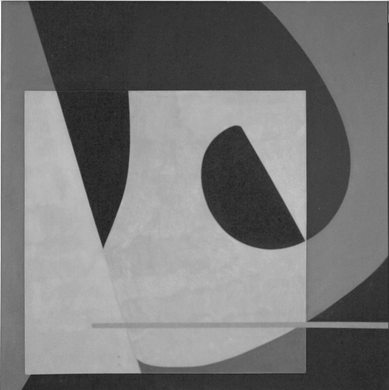
\includegraphics[scale=0.4]{part2/result/2_RGB_0.1_0.0_0.9_gray.png} \\
        \hline
    \end{tabular}
\end{table}

\clearpage

\begin{center}
    \textbf{(Describe the difference between those two grayscale images)}
\end{center}

Upon examining Table 4, it becomes apparent that the combination yielding a higher cost is $R*0.2+G*0.8+B*0.0(188019)$, while the one with a lower cost is $R*0.1+G*0.0+B*0.9(77882)$. Due to the variety of image color composition, direct observation via RGB colors poses a challenge to us. Nevertheless, through analyzing the fluctuation in grayscale luminance and subsequent texture alterations in RGB representation, we discern that the high-cost image, despite the noise has been removed, suffers from subdued color contrast across the entirety of the image. Conversely, the low-cost counterpart showcases enhanced contrast, facilitating a more distinct delineation of texture within the image.

\subsection{Describe how to speed up the implementation of bilateral filter}

From the definition, we have

\begin{align*}
    I^{\text{filtered}}(x) & ={\frac {1}{W_{p}}}\sum _{x_{i}\in \Omega }I(x_{i})f_{r}(\|I(x_{i})-I(x)\|)g_{s}(\|x_{i}-x\|)                                                  \\
    \Rightarrow g(x, y)    & ={\frac {1}{W_{p}}}\sum _{i, j\in[-r, r]}\underbrace{h_s(i, j)}_{\text{spatial kernel}}\underbrace{h_r(i, j)}_{\text{range kernel}}f(x-i, y-j) \\
    W_{p}                  & =\sum _{x_{i}\in \Omega }{f_{r}(\|I(x_{i})-I(x)\|)g_{s}(\|x_{i}-x\|)}                                                                          \\
    w(i,j,k,l)             & =d(i,j,k,l)\cdot r(i,j,k,l)                                                                                                                    \\
                           & =\exp\left(-{\frac {(i-k)^{2}+(j-l)^{2}}{2\sigma _{d}^{2}}}-{\frac {\|I(i,j)-I(k,l)\|^{2}}{2\sigma_{r}^{2}}}\right)                            \\
    I_{D}(i,j)             & ={\frac {\sum _{k,l}I(k,l)w(i,j,k,l)}{\sum _{k,l}w(i,j,k,l)}}                                                                                  \\
    h_s(i, j)              & =\exp^{-\frac{i^2+j^2}{2\sigma_s^2}}                                                                                                           \\
    h_r(i, j)              & =\exp^{-\frac{[f(x-i,y-j)-f(x,y)]^2}{2\sigma_r^2}}
\end{align*}

where

\hspace{2em}$I^{\text{filtered}}$ is the filtered image.

\hspace{2em}$I$ is the original input image.

\hspace{2em}$x$ are the coordinates of the current pixel to be filtered.

\hspace{2em}$\Omega$ is the window centered in $x$, so $x\in\Omega$ is another pixel.

\hspace{2em}$f_r$ is the range kernel for smoothing differences in intensities (Gaussian function).

\hspace{2em}$g_s$ is the spatial kernel for smoothing differences in coordinates (Gaussian function).

\hspace{2em}$W_{p}$ is the normalization term, also called weight.

\hspace{2em}$(i, j), (k, l)$ are the location of the pixel and the neighboring pixel.

\hspace{2em}$d(i, j, k, l), r(i, j, k, l)$ are the weight assigned for pixel $(i, j)$ and pixel $(k, l)$.

\hspace{2em}$I_d$ is the denoised intensity of pixel $(i, j)$

\hspace{2em}$\sigma_d, \sigma_r$ are smoothing parameters.

\vspace{1em}

Upon analyzing the properties of the equations provided above, the program efficiency can be optimized through three key strategies.

1. The coefficient of spatial distance $g_d(i, j, k, l)$ is independent of pixel values and solely relies on the matrix dimensions. Hence, precomputing and looking up when required offers optimization potential. \cite{5872028}

2. Optimizing grayscale value computation is imperative. Due to the large number of pixels, calculating each one individually incurs significant computational overhead. This indicates that the sheer volume of pixels necessitates a more efficient approach. Leveraging a lookup table for values within the $0-255$ range streamlines operations, obviating the need for individual computation, and it is good for efficient retrieval.

3. Streamlining the template from a two-dimensional to a one-dimensional format presents an opportunity for reducing algorithm complexity. This can be processed by refining the indexing mechanism, facilitating more streamlined processing.

\vspace{1em}

As a result, the optimization process can be implemented by calculating the look-up table of the range weights and spatial weights, followed by computing the total weight by producing them together and then calculating the weights based on different channels. After computing the weights, the code updates the result and weight matrices by accumulating the weighted pixel values and weights. Finally, the filtered output is obtained by dividing the accumulated result by the accumulated weight.

\section{Source code}
\subsection{Part 1 main.py}
\lstinputlisting[language=Python,breaklines=true,columns=flexible]{./part1/main.py}
\subsection{Part 1 DoG.py}
\lstinputlisting[language=Python,breaklines=true,columns=flexible]{./part1/DoG.py}
\subsection{Part 2 main.py}
\lstinputlisting[language=Python,breaklines=true,columns=flexible]{./part2/main.py}
\subsection{Part 2 JBF.py}
\lstinputlisting[language=Python,breaklines=true,columns=flexible]{./part2/JBF.py}

% BibTex
\bibliographystyle{ieeetr}
\bibliography{reference}

\end{document}